\subsection{\bt{Correctness after data changes}{数据变化后的正确性}}
\label{sec:changes-eval}
\label{sec:scenarios}
\label{sec:validity}
\bi{Shared knowledge can become stale as the database changes. We ask whether agents still answer correctly (Q3), including their own exploration when no usable definition remains.}
{共享知识可能随数据库变化而过期。我们检验智能体是否仍能正确作答（Q3），包括没有可用定义时转回自行探索的结果。}

\bi{\emph{After a restatement.} Following the population study, a restatement corrects store sales while retaining old amounts as non-current rows. Each of the \PpAgents\ agents returns with four affected questions. With each definition repaired once, \system\ answers \PpMavraChangeAcc\% correctly at \PpMavraChangeTokK\,k tokens per question; agents without memory answer \PpNoneChangeAcc\% at \PpNoneChangeTokK\,k. Trajectory Retrieval remains cheap (\PpTrajChangeTokK\,k) but answers \PpTrajChangeAcc\% correctly: its unmaintained SQL double-counts sales, and every wrong answer is \PpTrajChangeOverMin--\PpTrajChangeOverMax\% too high.}
{\emph{一次更正之后。}群体实验后，一次更正修改门店销售并将旧金额保留为非当前行。\PpAgents\ 个智能体各回来回答四道受影响的题。每个定义只修复一次后，\system\ 每题用 \PpMavraChangeTokK\,k token、答对 \PpMavraChangeAcc\%；无记忆智能体每题用 \PpNoneChangeTokK\,k token、答对 \PpNoneChangeAcc\%。轨迹检索仍便宜（\PpTrajChangeTokK\,k），但只答对 \PpTrajChangeAcc\%：未维护的 SQL 重复计入销售，每个错误答案均偏高 \PpTrajChangeOverMin--\PpTrajChangeOverMax\%。}

\bi{\emph{Eleven changes on two schemas.} Each run learns a library, then applies eleven changes independently to the initial data and library: four non-breaking updates, five targeted structural changes, and two outside-coverage changes (unit scaling and backup copies). Figure~\ref{fig:twoschemas} compares seven methods on synthetic retail and the three evaluated on TPC-H. It measures final answer accuracy, including fallback exploration. Supplementary Table S1 in the artifact retains held-out and all-setting results, separates unit and backup changes, and includes both regression variants.}
{\emph{两种模式上的十一种变化。}每次运行先学习定义库，再从初始数据与定义库分别施加十一种变化：四种正常更新、五种目标结构变化，以及单位缩放和备份副本两种范围外变化。图~\ref{fig:twoschemas} 比较合成零售数据的七种方法与 TPC-H 已评测的三种方法，衡量包含回退探索在内的最终答案正确率。工件中的补充表 S1 保留留出题与全部情形结果，分别报告单位和备份变化，并列出两个回归变体。}
\begin{figure}[t]
\centering
\ifbilingual
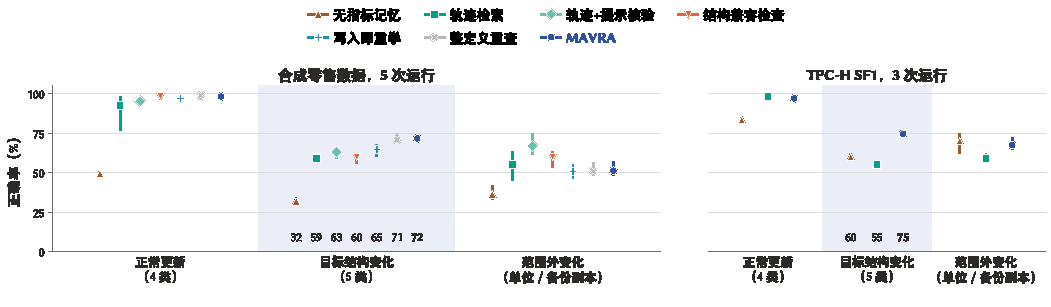
\includegraphics[width=\linewidth]{figures/two-schemas-zh}
\else
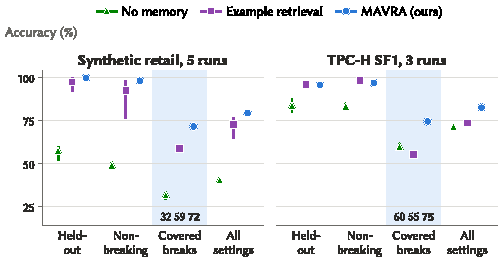
\includegraphics[width=\linewidth]{figures/two-schemas}
\fi
\caption{\bt{Accuracy over held-out questions, eleven changes and cross-agent forms (\PubScenarioScored{} answers). Equal-schema means across all \PubScenarioSettings{} settings: MAVRA \PubJointMAVRAAcc\%, AWM \PubJointAWMAcc\%. One run/method; frozen baseline controls reused.}{留出题、十一种变化及跨智能体题型的正确率（\PubScenarioScored{} 次作答）。两模式及全部 \PubScenarioSettings{} 种情形等权汇总：MAVRA \PubJointMAVRAAcc\%，AWM \PubJointAWMAcc\%。每方法一轮，复用冻结基线对照。}}
\label{fig:twoschemas}
\Description{Compact grouped bars compare ACE, AWM, G-Memory, and full MAVRA on synthetic retail and TPC-H SF1. Questions cover single periods, period differences, highest months and largest monthly increases. Groups show non-breaking updates, covered structural changes, new-agent form transfer, and all settings, on a common zero-to-100-percent scale. All settings also include the original held-out, unit and backup-source cases. Unchanged published baseline controls are reused; the repaired native method and all extra queries are freshly evaluated. Each extra question provides the same explicit business definition to a new agent. No confidence intervals or statistical-significance claim is made.}
\end{figure}


\bi{\emph{Maintenance beyond retrieval and prompting.} After non-breaking updates, \system\ retains high accuracy (\DsCondBenign\% on synthetic retail and \GeCondBenign\% on TPC-H); trajectory retrieval also remains effective. Targeted structural changes separate the methods: on synthetic retail, prompted verification improves retrieval from \DsTrajModeled\% to \DsTrajVerifyModeled\%, but remains below \system's \DsCondModeled\% by \DsCmpModeledCondVerify\ percentage points (95\% run-bootstrap interval: \DsCmpModeledCondVerifyLo\ to \DsCmpModeledCondVerifyHi). On TPC-H, \system\ reaches \GeCondModeled\% versus \GeTrajModeled\% for retrieval. Reminders to verify old SQL do not recover the accuracy observed with maintained definitions in this workload.}
{\emph{维护相对检索与核验提示的作用。}正常更新后，\system\ 保持较高正确率（合成零售数据 \DsCondBenign\%，TPC-H 为 \GeCondBenign\%），轨迹检索也仍然有效。目标结构变化拉开了方法差距：合成数据上，提示核验将检索的正确率从 \DsTrajModeled\% 提至 \DsTrajVerifyModeled\%，仍比 \system\ 的 \DsCondModeled\% 低 \DsCmpModeledCondVerify\ 个百分点（按运行自助抽样的 95\% 区间为 \DsCmpModeledCondVerifyLo\ 至 \DsCmpModeledCondVerifyHi）。TPC-H 上，\system\ 为 \GeCondModeled\%，轨迹检索为 \GeTrajModeled\%。在该负载中，提醒智能体核验旧 SQL 尚未达到维护定义所获得的正确率。}

\bi{\emph{Accuracy does not distinguish maintenance granularity.} Definition-Level Maintenance reaches \DsDefModeled\% on synthetic structural changes, with a \system\ advantage of only \DsCmpModeledDef\ percentage point (95\% interval: \DsCmpModeledDefLo\ to \DsCmpModeledDefHi). No accuracy difference is distinguishable here. Section~\ref{sec:cost} therefore measures the cost of checking and repair, using controlled maintenance workloads to examine the benefit of sharing that work.}
{\emph{正确率未区分维护粒度的收益。}整定义重查在合成数据的结构变化下达到 \DsDefModeled\%，\system\ 仅高 \DsCmpModeledDef\ 个百分点（95\% 区间为 \DsCmpModeledDefLo\ 至 \DsCmpModeledDefHi），没有可分辨的正确率差别。因此，第~\ref{sec:cost} 节进一步测量检查与修复代价，通过受控维护负载检验共享这些工作的收益。}

\bi{\emph{Limits of structural conditions.} The outside-coverage group shows no consistent advantage for \system. On synthetic backup copies, prompted verification reaches \DsTrajVerifyMirror\% versus \DsCondMirror\% for \system; on TPC-H, \system\ reaches \GeCondMirror\% on backup copies but only \GeCondUnit\% under unit scaling. Maintaining grain and joins does not resolve every value-semantic change or ambiguous repair. The fixed-library audit below separates incorrect reuse from conservative withdrawal.}
{\emph{结构条件的边界。}范围外变化中，\system\ 没有稳定优势。合成数据的备份副本下，提示核验达到 \DsTrajVerifyMirror\%，\system\ 为 \DsCondMirror\%；TPC-H 上，\system\ 在备份副本下达到 \GeCondMirror\%，单位缩放下却仅为 \GeCondUnit\%。维护粒度与连接不能解决所有值域语义变化或有歧义的修复。下面的固定库审计进一步区分错误复用与保守撤下。}

\begin{table}[t]
\caption{\bt{Fixed-library replay on TPC-DS, TPC-H, SSB, and BIRD financial: \RsTotal\ common question instances, \system\ with the learning-snapshot reference. Refusals are unavailable definitions, not correct answers; parentheses count refusals where the original SQL would still be correct.}{TPC-DS、TPC-H、SSB 与 BIRD financial 固定库回放：\RsTotal\ 个共同题次，\system\ 使用学习快照参照。拒绝表示定义不可用，不计为正确答案；括号内为原 SQL 仍能正确作答的拒绝。}}
\label{tab:replay-safety}
\centering
\footnotesize
\setlength{\tabcolsep}{3pt}
\begin{tabular}{@{}lrrr@{}}
\toprule
\bh{Change group}{变化分组} & \bh{Correct}{正确服务} & \bh{Wrong}{错误服务} & \bh{Refused}{拒绝}\\
\midrule
\bh{Non-breaking (4)}{正常更新（4 类）} & \RsBenignCorrect & \RsBenignWrong & \RsBenignRefused\ (\RsBenignUnneeded)\\
\bh{Targeted structural (5)}{目标结构变化（5 类）} & \RsStructuralCorrect & \RsStructuralWrong & \RsStructuralRefused\ (\RsStructuralUnneeded)\\
\bh{Unit / backup copy (2)}{单位／备份副本（2 类）} & \RsOutsideCorrect & \RsOutsideWrong & \RsOutsideRefused\ (\RsOutsideUnneeded)\\
\bottomrule
\end{tabular}
\end{table}

\bi{\emph{Preventing invalid reuse.} Table~\ref{tab:replay-safety} separates service from refusal on fixed-library replays over four benchmark databases. Across the five targeted structural scenarios, maintenance blocks \the\numexpr\RsStructuralRefused-\RsStructuralUnneeded\relax\ uses whose original SQL would be incorrect, with \RsStructuralWrong\ incorrect results served. A further \RsStructuralUnneeded\ uses are conservatively withheld because their conditions fail even though the original SQL still yields the reference answer. Revocation directs the agent to standard exploration. The unit/backup group marks the boundary between structural invariants and value semantics: \RsOutsideWrong/\RsOutsideN\ instances return incorrect results (43\% overall; 56\% of the \the\numexpr\RsOutsideCorrect+\RsOutsideWrong\relax\ served answers), and \RsOutsideRefused\ are refused. The two scenarios expose different requirements: unit scaling changes measure values while preserving grain and join cardinalities; an appended backup can violate grain yet leave multiple filters that each restore uniqueness. Future work will add unit-aware value checks and explicit source-of-record constraints to address these respective gaps.}
{\emph{阻止失效复用。}表~\ref{tab:replay-safety} 在四个基准数据库的固定库回放中区分服务与拒绝。五类目标结构变化中，维护阻止了 \the\numexpr\RsStructuralRefused-\RsStructuralUnneeded\relax\ 次原 SQL 会出错的使用，实际提供的错误结果为 \RsStructuralWrong\ 次。另有 \RsStructuralUnneeded\ 次使用虽仍能由原 SQL 得到参考答案，但因条件失效而被保守撤下。撤销引导智能体转入常规探索。单位／备份副本组标明结构不变性与值域语义的边界：\RsOutsideWrong/\RsOutsideN\ 个题次返回错误结果（占全部题次的 43\%；占 \the\numexpr\RsOutsideCorrect+\RsOutsideWrong\relax\ 个已服务答案的 56\%），另有 \RsOutsideRefused\ 次被拒绝。两种情形暴露不同的语义需求：单位缩放改变度量值，却保持粒度与连接基数；追加备份则可能破坏粒度，同时留下多个均能恢复唯一性的过滤。未来工作将分别引入感知量纲的值级检查与显式权威来源约束，补齐这两类缺口。}

\bi{All three structural-scenario errors come from one TPC-H Q12 definition. Its period uses \code{l\_receiptdate}, but its filter compares \code{l\_shipdate < l\_commitdate}. The date-key change appends rows with null \code{l\_shipdate}; receipt-date coverage still passes, while SQL's null comparison drops those rows. The September total is \RsQSingleObserved\ instead of \RsQSingleGold, the period difference is \RsQDiffObserved\ instead of \RsQDiffGold, and the highest month is \RsQRankObserved\ instead of \RsQRankGold. Extending completeness checks to the auxiliary filter columns \code{l\_shipdate} and \code{l\_commitdate}, alongside the primary date key \code{l\_receiptdate}, would detect this failure. In the concurrent grain-breaking stress test, same-snapshot validation prevents unsafe execution; precheck-then-execute admits up to \SnPreUnannMax\% unsafe queries.}
{三次结构变化情形下的错误均来自同一个 TPC-H Q12 定义。其期间使用 \code{l\_receiptdate}，过滤却比较 \code{l\_shipdate < l\_commitdate}。日期键变化追加了 \code{l\_shipdate} 为空的行；收货日期的覆盖检查仍通过，但 SQL 的空值比较排除了这些行。九月总量为 \RsQSingleObserved\ 而非 \RsQSingleGold，跨期差值为 \RsQDiffObserved\ 而非 \RsQDiffGold，最高月为 \RsQRankObserved\ 而非 \RsQRankGold。在主日期键 \code{l\_receiptdate} 之外，将完整性检查扩展至辅助过滤列 \code{l\_shipdate} 与 \code{l\_commitdate}，即可检测这一失效情形。在破坏粒度的并发压力测试中，同快照验证阻止不安全执行；先检查后执行最多有 \SnPreUnannMax\% 的查询使用失效数据。}
